\documentclass[12pt,a4paper]{article} 

\usepackage{fn2kursstyle}
\usepackage[russian]{babel}
\usepackage[T2A]{fontenc} 
\usepackage[utf8]{inputenc} 
\usepackage{geometry}
\usepackage{graphicx}
\usepackage{mathtools}
\usepackage{tikz}
\usepackage{pdfpages}
\usepackage{booktabs}
\usepackage{multirow,array}
\usepackage{siunitx}
\usepackage{amsmath}
\usepackage[hidelinks]{hyperref}
\usepackage{dblfloatfix}

\counterwithout{equation}{section}
\counterwithout{figure}{section}
\graphicspath{{pic/}}
\frenchspacing 

\newcolumntype{C}[1]{>{\centering\arraybackslash}p{#1}}

\newcommand{\picref}[1]{рис. \ref{#1}}
\newcommand{\tabref}[1]{таблица \ref{#1}}
\newcommand{\half}{\frac{1}{2}}
\newcommand{\dhalf}{\dfrac{1}{2}}
\newcommand*{\Scale}[2][4]{\scalebox{#1}{$#2$}}

\title{Упругие характеристики поликристаллических металлов \\ Вариант 15 \\ $\alpha$-Fe+Cd}
\group{ФН2-72Б}
\author{А.\,И.~Токарев}
\supervisor{И.\,Ю.~Савельева}
\date{2022}

\begin{document}
\maketitle
\tableofcontents
\newpage

\section-{Постановка задачи}

Для заданной пары чистых металлов ($\alpha$-$Fe$ -- железо, $Cd$ -- кадмий) по значению коэффициентов упругости (или податливости) кристаллов вычислить элементы матрицы коэффициентов податливости (или упругости), сравнив точность обращения матриц с вычислением по формулам, и построить графики зависимостей линейной податливости от направления единичного вектора для гексагональной кристаллической решетки в плоскости, содержащей оптическую ось кристалла, а для кубической кристаллической решетки в плоскости грани и в плоскостях, содержащих диагонали грани и куба. Для кристаллической решетки каждого из металлов определить направления, по которым линейная податливость имеет экстремальные значения. Найти отношение полуосей эллипсоида вращения, образующегося после действия всестороннего давления на шар из металла с ГПУ кристаллической решеткой.

Для каждого из металлов в предположении хаотической ориентации зерен в поликристалле найти верхнюю и нижнюю оценки продольной упругости и сравнить полученные значения с вычисленными для случая статистически усредненной шаровой формы кристаллических зерен. Провести аналогичные расчеты и построить графики для пористого двухфазного сплава-смеси заданной пары металлов при трех фиксированных значениях объемной пористости, равных 0; 0.1 и 0.2, в зависимости от отношения $\dfrac{V_1}{(V_1+V_2)}\in [0;1]$, где $V_1$ и $V_2$ --- объемные доли металлов в сплаве.

\begin{table}[htb!]
	\centering	
    \begin{tabular}{|c|c|c|c|}
        \hline
        $\alpha$-Fe & $C_{11}$ & $C_{12}$ & $C_{14}$ \\
        \hline
        ГПа & 234 & 135 & 114 \\
        \hline
    \end{tabular}
    \qquad
    \begin{tabular}{|c|c|c|c|c|c|}
        \hline
        Cd & $S_{11}$ & $S_{12}$ & $S_{13}$ & $S_{33}$ & $S_{44}$ \\
        \hline
        TПа$^{-1}$ & 12.4 & -0.76 & -9.97 & 37.5 & 63.7 \\
        \hline
    \end{tabular}
    \vspace*{3mm}
    \caption{Коэффициенты упругости и податливости}
    \label{tab1}
\end{table}

\newpage

\section-{Список условных обозначений}

\noindent\begin{tabular}{cp{0.7\textwidth}}

	$C$ & --- матрица коэффициентов упругости \\
	$C_{ij}$ & --- элементы матрицы $C$ $(i, j = \overline{1,6})$ \\
	$S$ & --- матрица коэффициентов податливости \\
	$S_{ij}$ & --- элементы матрицы $S$ $(i, j = \overline{1,6})$ \\
	$\vec{n} = \{n_1,n_2,n_3\}$ & --- единичный вектор нормали, заданный в кристаллографических осях. Компоненты $n_i$ --- проекции на $Ox^'_i$ \\
	$S_n$ & --- линейная податливость в направлении $\vec{n}$ \\
	$e^{(\vec n)}$ &--- относительное удлинение в направлении $\vec n$\\
	$\sigma_{kl}$ & ---  компоненты тензора напряжений $\hat{\sigma}$ $(k, l = \overline{1,3})$\\
	$S_{ijkl}$ & --- компоненты тензора податливости $\hat{S}$ $(i, j,k,l = \overline{1,3})$ \\
	$\varepsilon_{kl}$ & --- компоненты тензора малой деформации $\hat{\varepsilon}$ $(k, l = \overline{1,3})$\\
	$p$ & --- давление\\
	$\delta_{ij}$ & --- символ Кронекера \\
	$V_0$ & --- контрольный объем\\
	$I_{ijkl}$ & --- единичный тензор 4-го ранга $(i, j,k,l = \overline{1,3})$\\
	$\nu$ & --- коэффициент Пуассона\\
	$C_{ijkl}$ & --- компоненты тензора коэффициентов упругости $\hat{C}$ $(i, j,k,l = \overline{1,3})$ \\
	$C^o_{ijkl}$ & --- эффективные упругие характеристики поликристалла $(i, j,k,l = \overline{1,3})$ \\
	$S^o_{ijkl}$ & --- эффективные характеристики податливости поликристалла $(i, j,k,l = \overline{1,3})$ \\
	$\omega_{ijkl}$ & --- тензор Эшелби $(i, j,k,l = \overline{1,3})$\\
\end{tabular}

\newpage

\section{Матрицы податливости и упругости для различных типов решеток}

\subsection{Кубическая решетка}

В кристаллах с кубической решеткой матрицы коэффицентов податливости $S$ и упругости $C$ содержат лишь по $3$ независимых и отличных от нуля коэффициента:
\[
    C=
    \begin{pmatrix}
    C_{11} & C_{12} & C_{12} & 0 & 0 & 0\\
    C_{12} & C_{11} & C_{12} & 0 & 0 & 0\\
    C_{12} & C_{12} & C_{11} & 0 & 0 & 0\\
    0 & 0 & 0 & C_{44} & 0 & 0\\
    0 & 0 & 0 & 0 & C_{44} & 0\\
    0 & 0 & 0 & 0 & 0 & C_{44} 
    \end{pmatrix},  
\]
\\
\[
    S=
    \begin{pmatrix}
    S_{11} & S_{12} & S_{12} & 0 & 0 & 0\\
    S_{12} & S_{11} & S_{12} & 0 & 0 & 0\\
    S_{12} & S_{12} & S_{11} & 0 & 0 & 0\\
    0 & 0 & 0 & S_{44} & 0 & 0\\
    0 & 0 & 0 & 0 & S_{44} & 0\\
    0 & 0 & 0 & 0 & 0 & S_{44} 
    \end{pmatrix}.  
\]
\\
Обращение $С$ дает следующие расчетные формулы для ненулевых элементов матрицы $S\colon$
\[
    S_{11}=\frac{C_{11}+C_{12}}{C_K}, \quad S_{12}=-\frac{C_{12}}{C_K}, \quad S_{44}=\frac{1}{C_{44}}, \qquad C_K=(C_{11}-C_{12})(C_{11}+2C_{12}).  
\]

Пользуясь системой компьютерной алгебры Wolfram Mathematica, получим эти значения:
\[
    S_{11} = 7.4, \quad S_{12} = -2.7, \quad S_{13} = 8.8, \qquad S_{ij} = [\text{ТПа}^{-1}].
\]

Если вычислять эти коэффициенты путем обращения матрицы $C$, то можно оценить точность заданных формул:
\[
  \| S - C^{-1} \|  = 2 \cdot 10^{-27}
\]

\subsection{Гексагональная решетка}

В кристаллах с гексагональной решеткой в матрицах $S$ и $C$ уже присутствуют по $5$ независимых компонент:
\[
    S=
    \begin{pmatrix}
    S_{11} & S_{12} & S_{13} & 0 & 0 & 0\\
    S_{12} & S_{11} & S_{13} & 0 & 0 & 0\\
    S_{13} & S_{13} & S_{33} & 0 & 0 & 0\\
    0 & 0 & 0 & S_{44} & 0 & 0\\
    0 & 0 & 0 & 0 & S_{44} & 0\\
    0 & 0 & 0 & 0 & 0 & S_{66} 
    \end{pmatrix}.
\]
\\
\[
    C=
    \begin{pmatrix}
    C_{11} & C_{12} & C_{13} & 0 & 0 & 0\\
    C_{12} & C_{11} & C_{13} & 0 & 0 & 0\\
    C_{13} & C_{13} & C_{33} & 0 & 0 & 0\\
    0 & 0 & 0 & C_{44} & 0 & 0\\
    0 & 0 & 0 & 0 & C_{44} & 0\\
    0 & 0 & 0 & 0 & 0 & C_{66} 
    \end{pmatrix},
\]
\\
\noindent где $S_{66}=2(S_{11}-S_{12})$ и $C_{66}=\frac{1}{2}(C_{11}-C_{12})$. 

Обращение $S$ дает следующие расчетные формулы для ненулевых элементов матрицы $C\colon$
\[
    \begin{split}
        &C_{11}=\frac{S_{33}}{2 S_r}+\frac{1/2}{S_{11}-S_{12}}, \quad C_{12}=\frac{S_{33}}{2 S_r}-\frac{1/2}{S_{11}-S_{12}}, \quad C_{13}=-\frac{S_{13}}{S_r}, \quad  C_{33}=\frac{S_{11}+S_{12}}{S_r}, 
        \\[0.7em]
        &C_{44}=\frac{1}{S_{44}}, \quad C_{66}=\frac{1}{S_{66}}, \qquad S_r=(S_{11}+S_{12})S_{33}-2S_{13}^2.  
    \end{split}
\]

Вычисляя эти значения, получим:
\[
    \begin{split}
    C_{11} = 116.9, \quad C_{12} = 40.9, \quad C_{13}= 42, \quad C_{33} = 49, \quad C_{44} = 15.7, \quad &C_{66} = 38,
    \\
    & C = [\text{ГПа}].
    \end{split}
\]

А норма ошибки составляет:
\[
    \| C - S^{-1} \| = 1.5 \cdot 10^{-5}.
\]

\section{Зависимость линейной податливости
от направления единичного вектора}

Податливость кристаллов с кубическими решетками в направлении действия растягивающей или сжимающей силы равна:
\begin{gather}
    \label{podatCr}
    S_n=S_{11}-S_{44} (S^*-1)(n_1^2 n_2^2+n_2^2 n_3^2+n_3^2 n_1^2),
    \\[0.7em]
    S^*=2 \frac{S_{11}-S_{12}}{S_{44}}. \notag
\end{gather}

Из формулы \refeq{podatCr} видно, что при $S^* = 1$ податливость не зависит от направления силы.

Податливость кристаллов с ГПУ-решетками зависит от угла между оптической кристаллографической осью $Ox^'_3$ и направлением силы:
\begin{equation}
    S_n=S_{11} (1-n_3^2)+S_{33} n_3^4+(2 S_{13}+S_{44})n_3^2(1-n_3^2),   
\end{equation}
\noindent где $\vec n = (n_1, n_2, n_3)^T$ -- единичный вектор, определяющий направление силы.

\subsection{Линейная податливость для Cd (ГПУ)}

Рассмотрим случай, когда $\vec n$ лежит в плоскости, содержащей оптическую ось кристалла. Из этого следует, что $n_3 = \cos \gamma$, где $\gamma = \widehat{\bigl(\vec n, Ox^{'}_3 \bigr)}$, $\gamma \in \Bigl[ 0, \dfrac{\pi}{2} \Bigr]$.

\pagebreak

\begin{figure}[h]
	\center{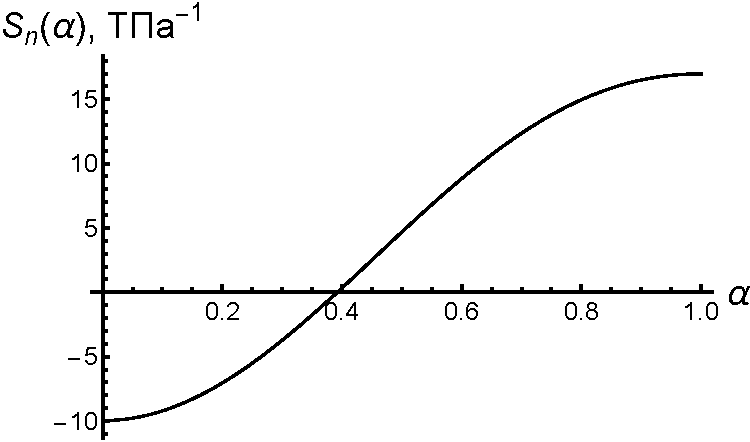
\includegraphics[width=0.8\textwidth]{II_1.pdf}}
	\caption{График линейной податливости в плоскости, содержащей оптическую ось кристалла}
	\label{pic:CdOpt}
\end{figure}

\subsection{Линейная податливость для $\alpha$-Fe (Кубическая кристаллическая решетка)}

\subsubsection{Единичный вектор в плоскости грани}

Есть три плоскости, содержащие начало координат кристаллографической системы:
\begin{enumerate}
	\item $\vec{n}\in \pi_1: \, n_3=0, \, n_1=\cos{\alpha}, \, n_2=\sin{\alpha}, \, \alpha \in \left[0; \, \dfrac{\pi}{2}\right]$.\\
	\item $\vec{n}\in \pi_2: \, n_2=0, \, n_1=\cos{\beta}, \, n_3=\sin{\beta}, \, \beta \in \left[0; \, \dfrac{\pi}{2}\right]$.\\
	\item $\vec{n}\in \pi_3: \, n_1=0, \, n_2=\cos{\gamma}, \, n_3=\sin{\gamma}, \, \gamma \in \left[0; \, \dfrac{\pi}{2}\right]$.\\
\end{enumerate}

Достаточно рассмотреть один из трех случаев. Выберем $\vec n \in \pi_1$. Подставив эти значения в (\refeq{podatCr}), получим:
\[
    S_n(\alpha) = S_n(\cos{\alpha},\sin{\alpha},0)=S_{11}-(2(S_{11}-S_{12})-S_{44}) \cos^2{\alpha} \sin^2{\alpha}.
\]

\pagebreak

\begin{figure}[h]
	\center{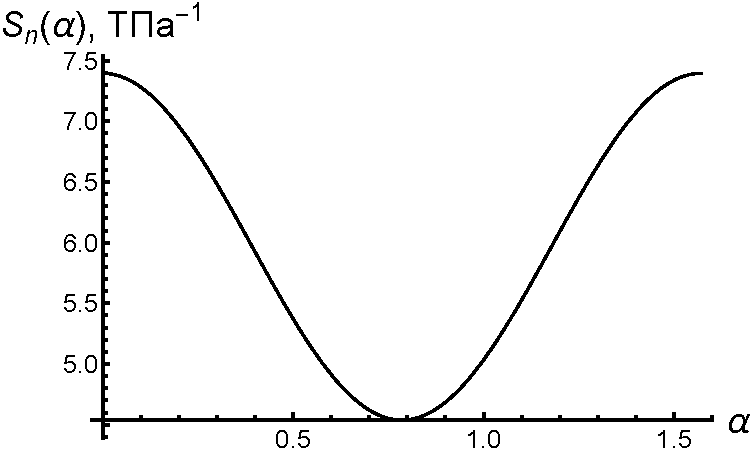
\includegraphics[width=0.8\textwidth]{I_1.pdf}}
	\caption{График линейной податливости в плоскости грани куба}
	\label{pic:FeOpt}
\end{figure}

\subsection{Вектор находится в плоскости, содержащей диагонали двух граней, имеющие общую точку}

Пусть первая диагональ лежит в лоскости $\pi_{2}$, вторая --- в $\pi_{3}$, а общая точка --- начало координат. Векторы $\vec{b_{1}}=\vec{i}+\vec{k},~~ \vec{b_{2}}=\vec{j}+\vec{k},$ лежат на этих диагоналях, следовательно, в рассматриваемой плоскости. Но не ортогональны, потому что $\cos{\widehat{\vec{b_{1}}, \vec{b_{2}}}}=\frac{1}{2}.$
Ортогонализируем по алгоритму Грама-Шмидта:

\begin{gather*}
\vec{e_{1}}=\frac{\vec{b_{1}}}{\|\vec{b_{1}}\|}=\sqrt{2}(\vec{i}+\vec{k}),
\end{gather*}

\begin{gather*}
	\vec{d_{2}}=\vec{b_{2}}-\langle \vec{e_{1}}, \vec{b_{2}} \rangle \vec{e_{1}}=-\frac{1}{2}\vec{i}+\vec{j}+\frac{1}{2}\vec{k},
 		\end{gather*}
		
\begin{gather*}
	\vec{e_{2}}=\frac{\vec{d_{2}}}{\|\vec{d_{2}}\|}=-\frac{1}{6}\vec{i}+\sqrt{\frac{2}{3}}\vec{j}+\frac{1}{\sqrt{6}}\vec{k}.
 		\end{gather*}

Тогда вектор $\vec{e_{3}}$ определим:
\begin{gather*}
	\vec{e_{3}}=\vec{e_{1}} \times \vec{e_{2}}=-\frac{1}{\sqrt{3}}\vec{i}-\frac{1}{\sqrt{3}}\vec{j}+\frac{1}{\sqrt{3}}\vec{k}.
\end{gather*}

\begin{gather*}
	A_{\mathcal{B} \rightarrow \mathcal{E}}=
	\begin{pmatrix}
  \frac{1}{\sqrt{2}} & -\frac{1}{\sqrt{6}} & -\frac{1}{\sqrt{3}}\\
  0 & \sqrt{\frac{2}{3}} & -\frac{1}{\sqrt{3}}\\
\frac{1}{\sqrt{2}} & \frac{1}{\sqrt{6}} & \frac{1}{\sqrt{3}}
\end{pmatrix} 
	\end{gather*}
 Тогда получим
 \begin{gather*}
		\begin{align}
			\begin{pmatrix}
				   n_{1} \\
				   n_{2} \\
				   n_{3}
				 \end{pmatrix} =
				 \begin{pmatrix}
					\frac{1}{\sqrt{2}}\cos{\alpha} -\frac{1}{\sqrt{6}}\sin{\alpha} \\
  \sqrt{\frac{2}{3}}\sin{\alpha}\\
  \frac{1}{\sqrt{2}}\cos{\alpha} + \frac{1}{\sqrt{6}}\sin{\alpha} 
\end{pmatrix}
 \end{align}
 \end{gather*}
 В случае, если $\pi \in \Bigl[0;~\dfrac{\pi}{3}\Bigr]$ вектор $\vec{n}$ расположен внутри куба и плоскости $-x_{1}-x_{2}+x_{3}=0.$ Получим зависимость:
 \[
	S_n(\alpha) = S_n \Bigl( \dfrac{1}{\sqrt 2} \cos \alpha - \dfrac{1}{\sqrt 6} \sin \alpha, \sqrt{\dfrac{2}{3}} \sin \alpha, \dfrac{1}{\sqrt 2} \cos \alpha + \dfrac{1}{\sqrt 6} \sin \alpha \Bigr).
 \] 

 \begin{figure}[h]
	\center{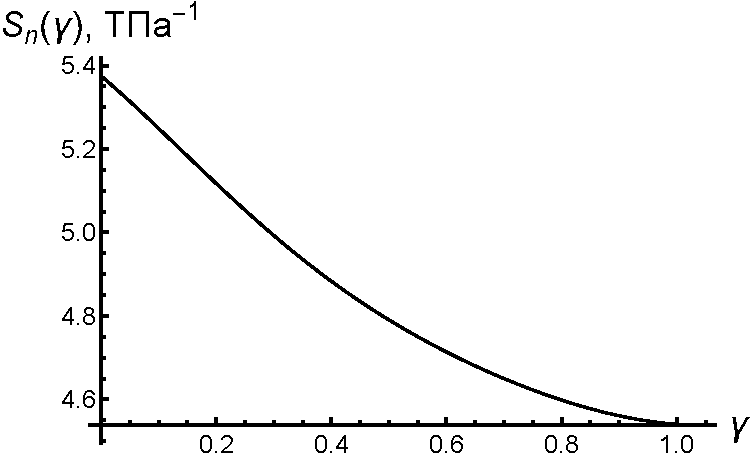
\includegraphics[width=0.8\textwidth]{I_2.pdf}}
	\caption{График $\S_n(\alpha), 0 \leq \alpha \leq \dfrac{\pi}{3}$}
	\label{pic:FeOpt2}
\end{figure}

 Получаем, что графиком функции является прямая, параллельная оси абсцисс. Полученный результат закономерен, так как $n_1^2 n_2^2 + n_2^2 n_3^2 + n_3^2 n_1^2 = \dfrac{1}{4}$.

 \subsection{Единичный вектор лежит в плоскости, содержащей диагонали грани и куба, имеющие общую точку}

 Пусть диагональ грани лежит в плоскости $\pi_3$, диагональ куба проходит через начало координат. Векторы $\vec b_1 = \vec i + \vec k, \vec b_2 = \vec i + \vec j + \vec k$ лежат на этих диагоналях, а следовательно и в рассматриваем плоскости. Но они не ортогональны, так как $ \cos{\Bigl(\widehat{\vec b_1, \vec b_2}\Bigr)} = \sqrt{\dfrac{2}{3}} $. Применим к ним процесс ортогонализации Грама-Шмидта.
 \[
	\vec e_1 = \dfrac{\vec b_1}{\| \vec b_1 \|} = \dfrac{1}{\sqrt 2}\bigl( \vec i + \vec k \bigr),
 \]
 \[
	\vec d_2 = \vec b_2 - \langle \vec e_1, \vec b_2 \rangle \vec e_1 = \vec j,
 \]
 \[
 	\vec e_2 = \vec j.
 \]

 Оставшийся вектор $\vec e_3$ определим из соотношения
 \[
	\vec e_3 = \vec e_1 \times \vec e_2 = \dfrac{1}{\sqrt 2}\Bigl( -\vec i + \vec k \Bigr)
 \]

 Выберем $\vec e_1, \vec e_2, \vec e_3 $ в качестве базиса $e$. Тогда
 \[
	\mathcal A_{\mathcal B \rightarrow \mathcal \Epsilon} = 
	\begin{pmatrix}
		\dfrac{1}{\sqrt 2} & 0 & -\dfrac{1}{\sqrt 2} \\ 
		0 & 1 & 0 \\
		\dfrac{1}{\sqrt 2} & 0 & \dfrac{1}{\sqrt 2}
	\end{pmatrix},
 \]

 \[
	\begin{pmatrix}
		n1 \\
		n2 \\
		n3	
	\end{pmatrix} = \begin{pmatrix}
		\dfrac{1}{\sqrt 2} \cos \alpha \\
		\sin \alpha \\
		\dfrac{1}{\sqrt 2} \cos \alpha
	\end{pmatrix}.
 \]

 При $\alpha \in \Bigr[ 0, \dfrac{\pi}{2} \Bigl]$ вектор $ \vec n $ расположен внутри куба в плоскости $ -x_1 + x_3 = 0 $. Получим зависимость 
 \[
	S_n(\alpha) = S_n \Bigl( \dfrac{1}{\sqrt 2} \cos \alpha, \sin \alpha, \dfrac{1}{\sqrt 2} \cos \alpha \Bigr).
 \] 

 \begin{figure}[h]
	\center{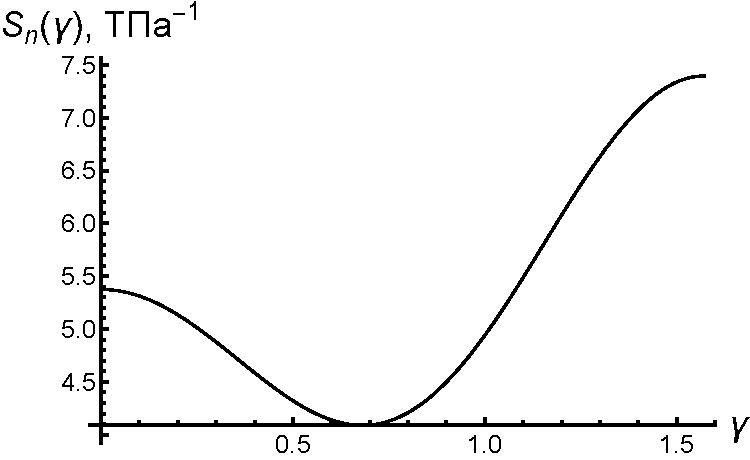
\includegraphics[width=0.8\textwidth]{I_3.pdf}}
	\caption{График $S_n(\alpha), 0 \leq \alpha \leq \dfrac{\pi}{2}$}
	\label{pic:FeOpt3}
\end{figure}

 \subsection{Единичный вектор лежит в плоскости, содержащей диагональ куба и ребро, имеющие общую точку}

 Пусть диагональ куба проходит через начало координат, ребро лежит на оси $x_1.$ Векторы $ \vec e_1 = \vec i, \vec b_2 = \vec i + \vec j + \vec k $ лежат на ребре и диагонали соответсвенно, а следовательно, и в рассматриваемой плоскости. Но они не ортогональны, так как $\cos{\Bigl( \widehat{\vec e_1, \vec b_2} \Bigr)} = \dfrac{1}{\sqrt 3}$. Применим к ним процесс ортогонализации Грама-Шмидта: 
 \[
	\vec d_2 = \vec b_2 - \langle \vec e_1, \vec b_2 \rangle \vec e_1 = \vec j + \vec k,
 \]
\[
	\vec e_2 = \dfrac{1}{\sqrt 2}\Bigl(\vec j + \vec k \Bigr).	
\]

Оставшийся вектор $\vec e_3$ определим из соотношения 
\[
	\vec e_3 = \vec e_1 \times \vec e_2 = \dfrac{1}{\sqrt 2}\Bigl(\vec j + \vec k\Bigr).	
\]

Выберем $\vec e_1, \vec e_2, \vec e_3 $ в качестве базиса $\mathcal \Epsilon$. Тогда 
\[
	\mathcal A_{\mathcal B \rightarrow \mathcal \Epsilon} = \begin{pmatrix}
		1 & 0 & 0 \\
		0 & \dfrac{1}{\sqrt 2} & -\dfrac{1}{\sqrt 2} \\[1em]
		0 & \dfrac{1}{\sqrt 2} & \dfrac{1}{\sqrt 2}	
	\end{pmatrix},
\]

\[
	\begin{pmatrix}
		n1 \\
		n2 \\
		n3	
	\end{pmatrix} = \begin{pmatrix}
		\cos \alpha \\[0.2em]
		\dfrac{1}{\sqrt 2} \sin \alpha \\[1em]
		\dfrac{1}{\sqrt 2} \sin \alpha
	\end{pmatrix}.
 \]

 При $\alpha \in \Bigr[ 0, \dfrac{\pi}{2} \Bigl]$ вектор $ \vec n $ расположен внутри куба в плоскости $ -x_2 + x_3 = 0 $. Получим зависимость 
 \[
	S_n(\alpha) = S_n \Bigl( \cos \alpha, \dfrac{1}{\sqrt 2} \sin \alpha, \dfrac{1}{\sqrt 2} \sin \alpha \Bigr).
 \] 

 \begin{figure}[h]
	\center{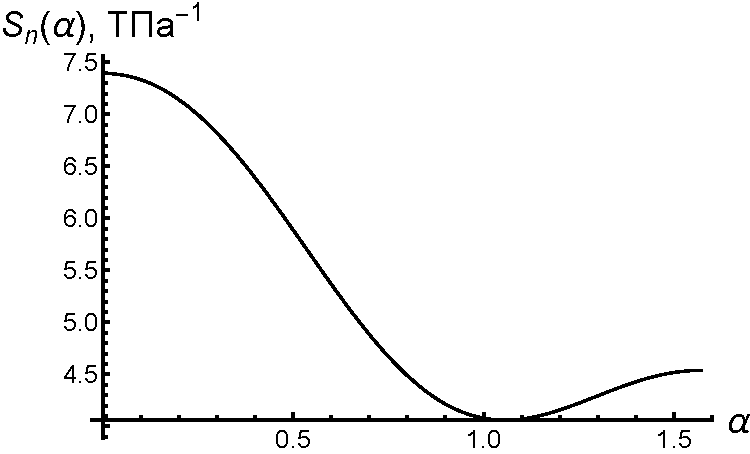
\includegraphics[width=0.8\textwidth]{I_4.pdf}}
	\caption{График $S_n(\alpha), 0 \leq \alpha \leq \dfrac{\pi}{2}$}
	\label{pic:FeOpt4}
\end{figure}

 Рассмотренная в предыдущем разделе плоскость удовлетворяет условиям этого пункта, то есть \picref{pic:FeOpt3} подходит и для рассматриваемого в данном пункте случая. Заметим, что если повернуть плоскость \picref{pic:FeOpt4} на угол $\pi$ по оси, совпадающей с осью $OS_n$, то с помощью преобразования параллельного переноса можно совместить кривые на \picref{pic:FeOpt4}.

 \section{Экстремальные значения линейной податливости}

 

 \section{Отношение полуосей эллипсоида вращения, образующегося путем всестороннего сжатия шара из металла с ГПУ решеткой}

 Напряжение и деформации при всестороннем сжатии:
 \[
   \sigma_{ij} = - p \delta_{ij}, \quad \varepsilon_{ij} = S_{ijkl} \sigma_{kl} = -p S_{ijkl} \delta_{kl} = -p S_{ijkk}.
 \]

 Деформация в направлении вектора, заданного в кристаллографических осях:
 \[
    \varepsilon_{ij} n_i n_j = -p S_{ijkk} n_i n_j,
 \]  
 \noindent откуда выражается коэффициент линейной сжимаемости кристалла:
 \[
    \beta_n = - \dfrac{\varepsilon_{ij}}{p} = S_{ijkk} n_i n_j = \sum \limits_{i, j = 1}^{3} S_{ij} n_i^2
 \]

 Пусть изначально шар имел радиус $R$. Найдем относительное удлинение вдоль осей координат $Ox_1^', Ox_3^'\colon$
 \[
    \begin{cases}
        \dfrac{\Delta R_1}{R} = -p S_{1j} n_1^2 = -p (S_{11} + S_{12} + S_{13}) = -1.67p, \\[0.7em]
        \dfrac{\Delta R_3}{R} = -p S_{i3} n_1^2 = -p (S_{31} + S_{32} + S_{33}) = -17.56p.
    \end{cases} \Rightarrow \dfrac{R_1}{R_3} = \dfrac{R + \Delta R_1}{R + \Delta R_3} = \dfrac{1 - 17.56p}{1 - 1.67p}
 \]

 \section{Верхняя и нижняя оценки параметров $\kappa$, $\mu$, $E$, $\nu$}

 Для изотропных сред известно:
 \begin{gather*}
    \kappa = \dfrac{1}{9}C^0_{iikk}, \quad \dfrac{1}{\kappa} = S^0_{iikk}, \qquad i, k = 1, 2, 3,
    \\[0.7em]
    \mu = \dfrac{1}{10}\Bigl( C^0_{ikik} - \dfrac{1}{3}C^0_{iikk} \Bigr), \quad \dfrac{1}{\mu} = \dfrac{2}{5}\Bigl( S^0_{ikik} - \dfrac{1}{3} S^0_{iikk} \Bigr), \qquad i, k = 1, 2, 3,
    \\[0.7em]
    \dfrac{1}{E} = \dfrac{1}{9 \kappa} + \dfrac{1}{3\mu}, \quad \nu = \dfrac{E}{2\mu} - 1.
 \end{gather*}

 Данные выражения можно упростить, группируя парные индексы:
 \[
    \begin{split}
        &C_{iikk} = C_{11} + C_{22} + C_{33} + 2C_{12} + 2C_{13} + 2C_{23},
        \\
        &C_{ikik} = C_{11} + C_{22} + C_{33} + 2C_{66} + 2C_{55} + 2C_{44},
        \\
        &S_{iikk} = S_{11} + S_{22} + S_{33} + 2S_{12} + 2S_{13} + 2S_{23},
        \\
        &S_{ikik} = S_{11} + S_{22} + S_{33} + \dfrac{S_{66}}{2} + \dfrac{S_{55}}{2} + \dfrac{S_{44}}{2}.
    \end{split}
 \]

 \subsection{Кубичесукая кристаллическая решетка}
 \begin{gather*}
    \kappa^+ = \dfrac{1}{3}(C_{11} + C_{12}), \quad \dfrac{1}{\kappa^-} = 3(S_{11} + 2S_{12}),
    \\[0.7em]
    \mu^+ = \dfrac{1}{5}(C_{11} - C_{12} + 3C_{44}), \quad \dfrac{1}{\mu^-} = \dfrac{1}{5}(4(S_{11} - S_{12} + 3S_{44}),
    \\[0.7em]
    E^+ = \dfrac{1}{\tfrac{1}{9 \kappa^-} + \tfrac{1}{3\mu^-}}, \quad E^- = \dfrac{1}{\tfrac{1}{9 \kappa^+} + \tfrac{1}{3\mu^+}},
    \\[0.7em]
    \nu^+ = \dfrac{E^-}{2\mu^-} - 1, \quad \nu^- = \dfrac{E^+}{2\mu^+} - 1.
 \end{gather*}

 Для $\alpha$-Fe эти величины равны соответственно:
 \begin{table}[h!]
    \centering
    \begin{tabular}{|c|c|c|c|c|c|c|c|}
        \hline 
        $\kappa^-$ & $\kappa^+$ & $\mu^-$ & $\mu^+$ & $E^-$ & $E^+$ & $\nu^-$ & $\nu^+$ \\
        \hline 
        $168.0$ & $168.0$ & $74.94$ & $88.2$ & $195.7$ & $225.2$ & $0.28$ & $0.305$ \\
        \hline
    \end{tabular}
    \vspace{3mm}
    \caption{Оценка параметров Ламе, модуля упругости и коэффициента Пуассона для железа}
 \end{table}

 \subsection{ГПУ}
 \begin{gather*}
    \kappa^+ = \dfrac{1}{9}(2C_{11} + C_{33} + 2(C_{12} + 2C_{13})), \quad \dfrac{1}{\kappa^-} = 2(S_{11} + 2S_{12}),
    \\[0.7em]
    \mu^+ = \dfrac{1}{30}(7C_{11} - 5C_{12} - 4C_{13} + 2C_{33} + 12C_{44}), \quad \dfrac{1}{\mu^-} = \dfrac{2}{15}(7S_{11} + 2S_{33} + 3S_{44} - 5S_{12} - 4S_{13}),
    \\[0.7em]
    E^+ = \dfrac{1}{\tfrac{1}{9 \kappa^-} + \tfrac{1}{3\mu^-}}, \quad E^- = \dfrac{1}{\tfrac{1}{9 \kappa^+} + \tfrac{1}{3\mu^+}},
    \\[0.7em]
    \nu^+ = \dfrac{E^-}{2\mu^-} - 1, \quad \nu^- = \dfrac{E^+}{2\mu^+} - 1.
 \end{gather*}

 \pagebreak

 Для Cd эти величины равны соответственно: 
 \begin{table}[h!]
    \centering
    \begin{tabular}{|c|c|c|c|c|c|c|c|}
        \hline 
        $\kappa^-$ & $\kappa^+$ & $\mu^-$ & $\mu^+$ & $E^-$ & $E^+$ & $\nu^-$ & $\nu^+$ \\
        \hline 
        $47.85$ & $64.58$ & $18.9$ & $25.8$ & $50.13$ & $68.3$ & $0.323$ & $0.325$ \\
        \hline
    \end{tabular}
    \vspace{3mm}
    \caption{Оценка параметров Ламе, модуля упругости и коэффициента Пуассона для железа}
 \end{table}

 \section{Задача Эшелби}

 Для оценки характеристик поликристаллического материала можно использо-
вать решение задачи Эшелби о взаимодействии с изотропной линейно-упругой сплошной средой изотропного линейно-упругого сферического или эллипсоидального включения. Для это необходимо решить систему уравнений:
\begin{equation}
    \begin{cases}
        \zeta_{kkmm} = 0, \\
        \zeta_{kmkm} = 0,
    \end{cases}  
    \label{eq:zeta}
\end{equation}

\noindent где 
\begin{gather*}
    \begin{split}
        \zeta_{ijmn} &= \dfrac{C_{rsmn}^0 - C_{rsmn}}{C_{ijrs} - C_{ijpq}^0 (I_{pqrs} - w_{pqrs})}, \\[0.7em]
        I_{ijkl} &= \dfrac{1}{2}(\delta_{ik} \delta_{jl} + \delta_{il} \delta_{jk}), \\[0.7em]
        w_{ijkl} &= \dfrac{\kappa + \frac{4 \mu}{3}}{2(\kappa + 2\mu)} \Bigl(\dfrac{4 \mu - 3\kappa}{3 \kappa} \delta_{ij} \delta_{kl} + 5 I_{ijkl} \Bigr), \\[0.7em]
        C^0_{11} &= \kappa + \dfrac{4 \mu}{3}, \quad C^0_{12} = \kappa - \dfrac{2\mu}{3}, \quad C^0_{44} = \mu.
    \end{split}
\end{gather*}

Необходимо представить тензор (\refeq{eq:zeta}) в виде матрицы:
\[
    \begin{cases}
        \zeta_{kkmm} = \zeta_{11} + \zeta_{22} + \zeta_{33} + 2(\zeta_{12} + \zeta_{13} + \zeta_{23}), \\
        \zeta_{kmkm} = \zeta_{11} + \zeta_{22} + \zeta_{33} + 2(\zeta_{44} + \zeta_{55} + \zeta_{66}),
    \end{cases}  
\]

\noindent чтобы найти его компоненты путем решения задачи минимизации:
\begin{equation}
    \zeta^2_{kkmm}(\kappa, \mu) + \zeta^2_{kmkm}(\kappa, \mu) \rightarrow \min.
    \label{eq:min}    
\end{equation}

\pagebreak

\begin{table}[h!]
    \centering
    \begin{tabular}{|c|c|c|c|c|}
        \hline 
        Металл & $ \kappa^{min}$ & $\mu^{min}$ & $E^{min}$ & $\nu^{min}$ \\
        \hline 
        Fe & $168$ & $83.4$ & $214.7$ & $0.286$ \\
        \hline
        Cd & $55$ & $22.13$ & $59.5$ & $0.322$ \\
        \hline 
    \end{tabular}
    \vspace{3mm}
    \caption{Оценка параметров Ламе, модуля упругости и коэффициента Пуассона для железа –- задача Эшелби}
 \end{table}

 \section{Задача с пористым двухфазным сплавом-смесью}

 Проведем аналогичные расчеты и построим графики для пористого двухфазного сплава-смеси пары металлов Fe и Cd при фиксированных значениях объемной пористости в зависимости от отношения $V1/(V1 + V2) \in [0, 1]$, где $V1$ и $V2$ -- объемные доли железа и кадмия в сплаве соответственно, $V3$ — объемная пористость, $V1 + V2 + V3 = 1$.

    \begin{figure}[h]
        \center{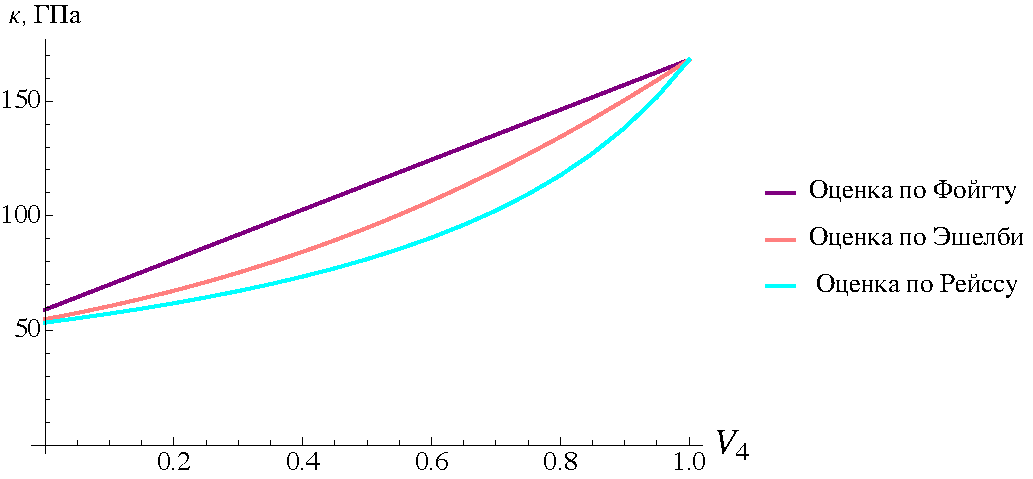
\includegraphics[width=\textwidth, height=0.45\textwidth]{lambdaj0.pdf}}
        \caption{График $\kappa(V_4), V_3 = 0$}
    \end{figure}

    \pagebreak

    \begin{figure}[h]
        \center{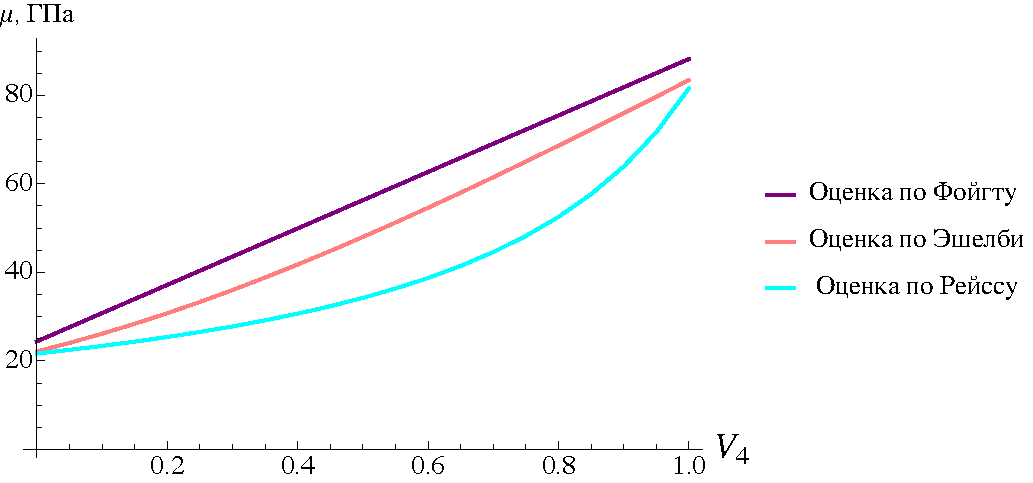
\includegraphics[width=\textwidth, height=0.45\textwidth]{muj0.pdf}}
        \caption{График $\mu(V_4), V_3 = 0$}
    \end{figure}

    \begin{figure}[h]
        \center{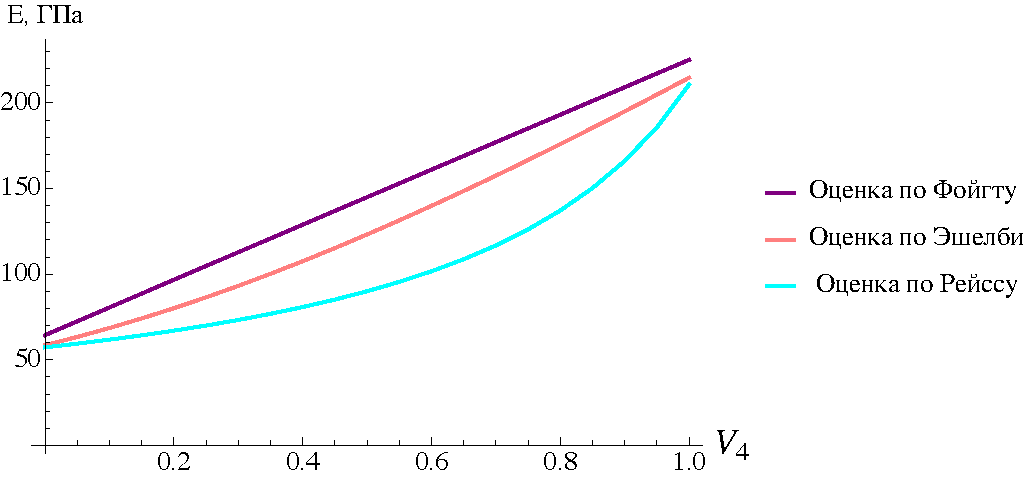
\includegraphics[width=\textwidth, height=0.45\textwidth]{Ej0.pdf}}
        \caption{График $E(V_4), V_3 = 0$}
    \end{figure}

    \pagebreak

    \begin{figure}[h]
        \center{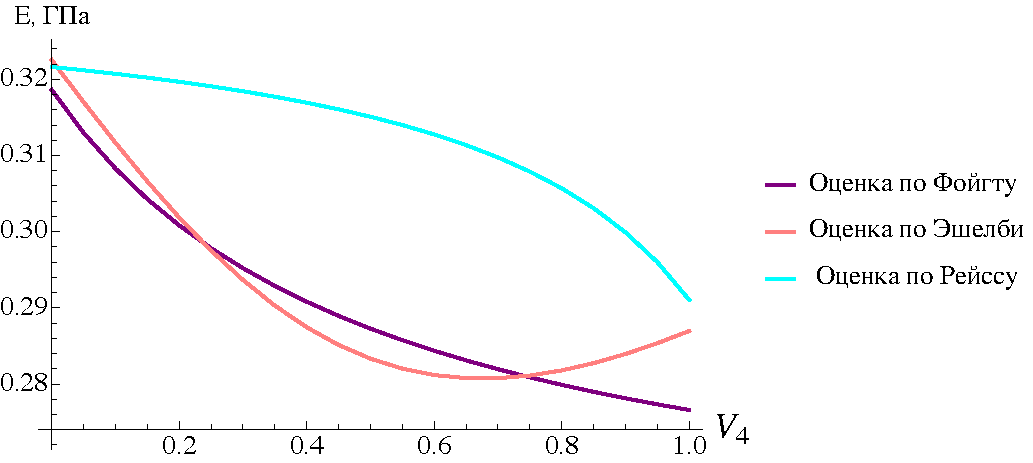
\includegraphics[width=\textwidth, height=0.45\textwidth]{nuj0.pdf}}
        \caption{График $\nu(V_4), V_3 = 0$}
    \end{figure}

    \begin{figure}[h]
        \center{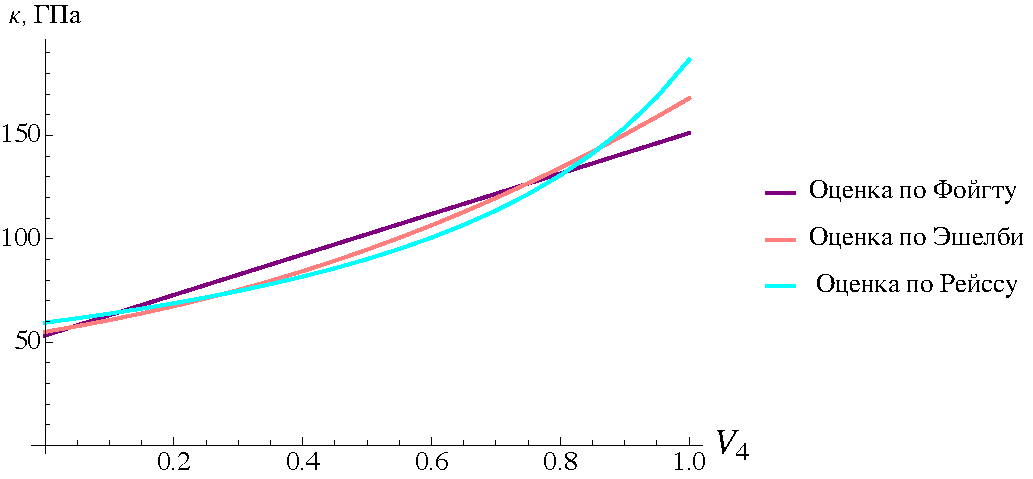
\includegraphics[width=\textwidth, height=0.45\textwidth]{lambdaj1.pdf}}
        \caption{График $\kappa(V_4), V_3 = 0.1$}
    \end{figure}

    \pagebreak

    \begin{figure}[h]
        \center{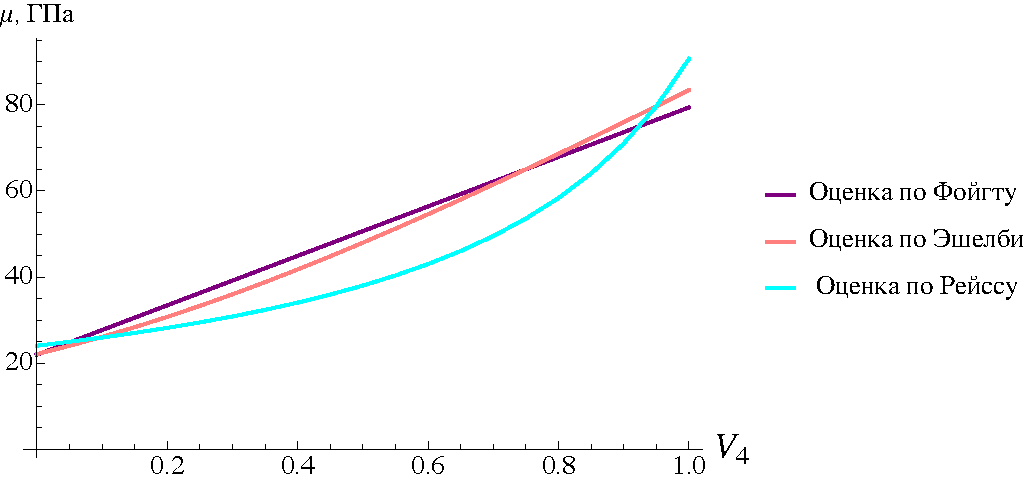
\includegraphics[width=\textwidth, height=0.45\textwidth]{muj1.pdf}}
        \caption{График $\mu(V_4), V_3 = 0.1$}
    \end{figure}

    \begin{figure}[h]
        \center{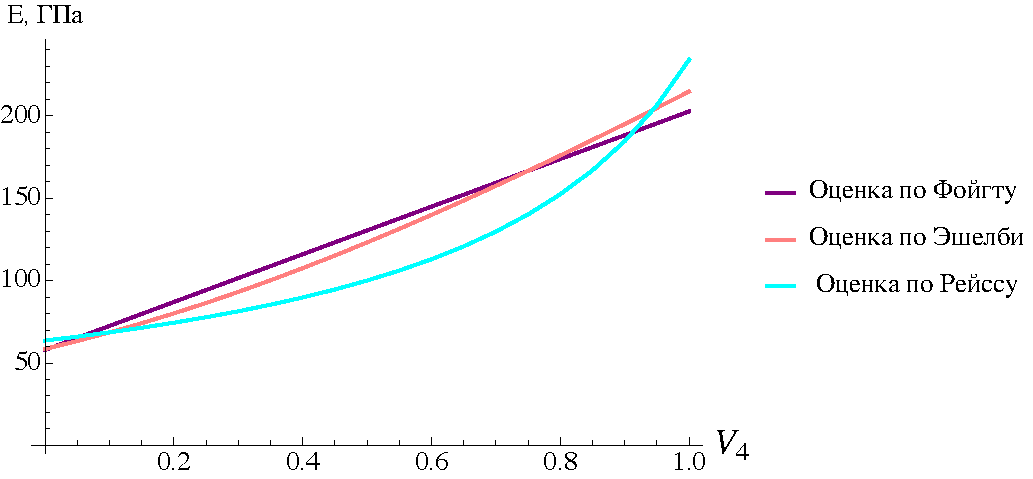
\includegraphics[width=\textwidth, height=0.45\textwidth]{Ej1.pdf}}
        \caption{График $E(V_4), V_3 = 0.1$}
    \end{figure}

    \pagebreak

    \begin{figure}[h]
        \center{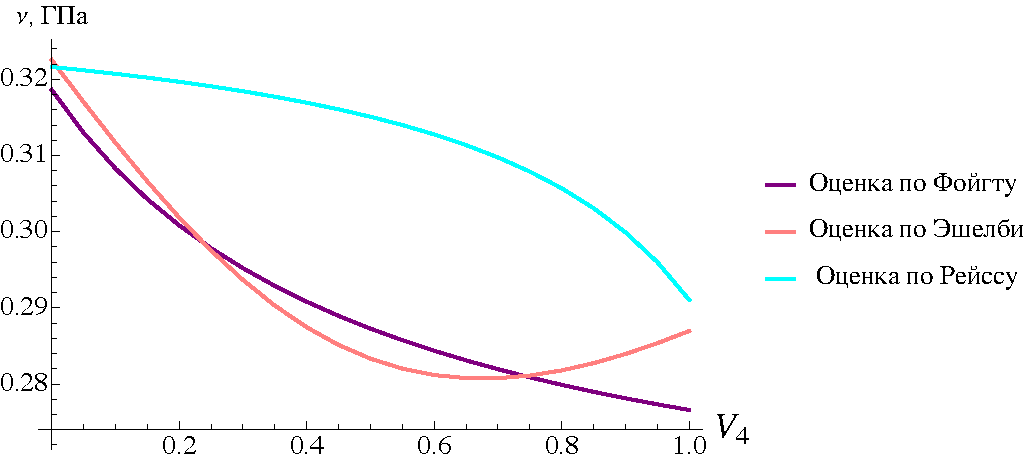
\includegraphics[width=\textwidth, height=0.45\textwidth]{nuj1.pdf}}
        \caption{График $\nu(V_4), V_3 = 0.1$}
    \end{figure}

    \section{Заключение}

    Для заданной пары металлов были вычислены коэффициенты матриц упругости и податливости с приведением сравнения точности. Построили графики зависимостей линейной податливости от направления единичного вектора в различных плоскостях для гексагональной плотной упако- ванной и кубической решеток, определена линия, вдоль которой линейная податливость имеет экстремальные значения. Для каждого из металлов в предположении хаотической ориентации зерен в поликристалле найдены верхняя и нижняя оценки модуля объемной упруго- сти и проведено сравнение полученных значений с вычисленными для случая статистически усредненной шаровой формы кристаллических зерен. Найдены верхняя и нижняя оценки модуля объемной упругости и построены графики для пористого двухфазного сплава-смеси заданной пары металлов при различных значениях объемной пористости. Рассмотрели отношения удлинения вдоль осей для металла с ГПУ решеткой.

\begin{thebibliography}{6}
\bibitem{zarkuv}	Зарубин В.С. Математические модели механики и электродинамики сплошной среды. [Текст]/ В.С. Зарубин, Г.Н. Кувыркин -- Москва: Издательство МГТУ им. Н.Э. Баумана, 2008. -- 512~с.
\bibitem{zar} Зарубин В.С. Прикладные задачи термопрочности элементов конструкций. [Текст] -- Москва: Машиностроение, 1985. -- 296 с.  
\bibitem{zarkuvsav} Зарубин В.С. Физические и математические модели микромеханики: учебное пособие. [Текст]/ В.С. Зарубин, Г.Н. Кувыркин, И.Ю. Савельева -- Москва: Москва: Издательство МГТУ им. Н.Э. Баумана, 2020. -- 194 с.
\end{thebibliography}

\end{document}